

\tikzset{every picture/.style={line width=0.75pt}} %set default line width to 0.75pt        

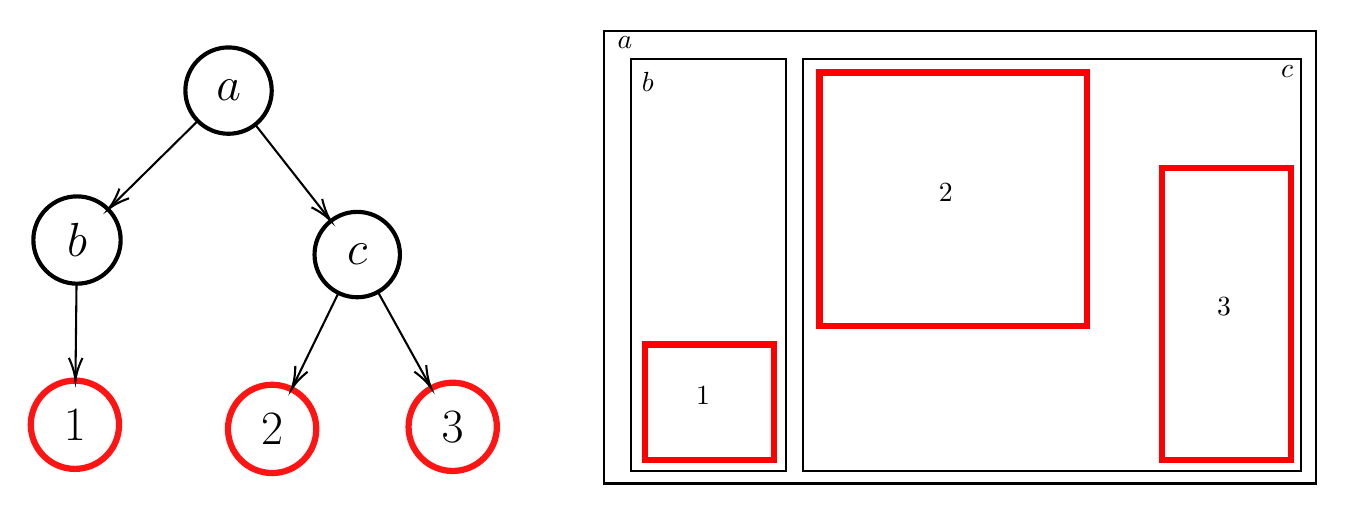
\begin{tikzpicture}[x=0.75pt,y=0.75pt,yscale=-1,xscale=1]
%uncomment if require: \path (0,269); %set diagram left start at 0, and has height of 269

%Shape: Rectangle [id:dp45712367712220003] 
\draw   (314,16.5) -- (657,16.5) -- (657,234.5) -- (314,234.5) -- cycle ;
%Shape: Rectangle [id:dp4249683313230568] 
\draw   (327,30) -- (402,30) -- (402,228.5) -- (327,228.5) -- cycle ;
%Shape: Rectangle [id:dp35105668268883494] 
\draw   (410,30) -- (650,30) -- (650,228.5) -- (410,228.5) -- cycle ;
%Shape: Rectangle [id:dp8308248735679132] 
\draw  [color={rgb, 255:red, 255; green, 0; blue, 0 }  ,draw opacity=1 ][line width=2.25]  (334,167.5) -- (396,167.5) -- (396,223) -- (334,223) -- cycle ;
%Shape: Rectangle [id:dp6177381470864712] 
\draw  [color={rgb, 255:red, 255; green, 0; blue, 0 }  ,draw opacity=1 ][line width=2.25]  (418,36.5) -- (547,36.5) -- (547,158.5) -- (418,158.5) -- cycle ;
%Shape: Rectangle [id:dp3774907556728889] 
\draw  [color={rgb, 255:red, 255; green, 0; blue, 0 }  ,draw opacity=1 ][line width=2.25]  (583,82.5) -- (645,82.5) -- (645,223) -- (583,223) -- cycle ;

% Text Node
\draw  [color={rgb, 255:red, 0; green, 0; blue, 0 }  ,draw opacity=1 ][line width=1.5]   (195.23, 124.2) circle [x radius= 20.57, y radius= 20.57]   ;
\draw (195.23,124.2) node  [font=\LARGE]  {$c$};
% Text Node
\draw  [color={rgb, 255:red, 0; green, 0; blue, 0 }  ,draw opacity=1 ][line width=1.5]   (60.22, 117.2) circle [x radius= 21.03, y radius= 21.03]   ;
\draw (60.22,117.2) node  [font=\LARGE]  {$b$};
% Text Node
\draw  [color={rgb, 255:red, 0; green, 0; blue, 0 }  ,draw opacity=1 ][line width=1.5]   (133.23, 45.2) circle [x radius= 20.8, y radius= 20.8]   ;
\draw (133.23,45.2) node  [font=\LARGE]  {$a$};
% Text Node
\draw  [color={rgb, 255:red, 255; green, 20; blue, 20 }  ,draw opacity=1 ][line width=2.25]   (59.22, 206.2) circle [x radius= 21.27, y radius= 21.27]   ;
\draw (59.22,206.2) node  [font=\LARGE]  {$1$};
% Text Node
\draw  [color={rgb, 255:red, 255; green, 20; blue, 20 }  ,draw opacity=1 ][line width=2.25]   (154.23, 208.2) circle [x radius= 21.27, y radius= 21.27]   ;
\draw (154.23,208.2) node  [font=\LARGE]  {$2$};
% Text Node
\draw  [color={rgb, 255:red, 255; green, 20; blue, 20 }  ,draw opacity=1 ][line width=2.25]   (241.23, 207.2) circle [x radius= 21.27, y radius= 21.27]   ;
\draw (241.23,207.2) node  [font=\LARGE]  {$3$};
% Text Node
\draw (324.23,22.2) node    {$a$};
% Text Node
\draw (335.23,41.2) node    {$b$};
% Text Node
\draw (643.23,36.2) node    {$c$};
% Text Node
\draw (357,186.4) node [anchor=north west][inner sep=0.75pt]    {$1$};
% Text Node
\draw (474,88.4) node [anchor=north west][inner sep=0.75pt]    {$2$};
% Text Node
\draw (608,143.4) node [anchor=north west][inner sep=0.75pt]    {$3$};
% Connection
\draw    (186.2,142.69) -- (164.44,187.28) ;
\draw [shift={(163.56,189.08)}, rotate = 296.02] [color={rgb, 255:red, 0; green, 0; blue, 0 }  ][line width=0.75]    (10.93,-3.29) .. controls (6.95,-1.4) and (3.31,-0.3) .. (0,0) .. controls (3.31,0.3) and (6.95,1.4) .. (10.93,3.29)   ;
% Connection
\draw    (205.2,142.2) -- (229.94,186.84) ;
\draw [shift={(230.91,188.59)}, rotate = 241] [color={rgb, 255:red, 0; green, 0; blue, 0 }  ][line width=0.75]    (10.93,-3.29) .. controls (6.95,-1.4) and (3.31,-0.3) .. (0,0) .. controls (3.31,0.3) and (6.95,1.4) .. (10.93,3.29)   ;
% Connection
\draw    (146.07,61.56) -- (181.29,106.44) ;
\draw [shift={(182.52,108.02)}, rotate = 231.87] [color={rgb, 255:red, 0; green, 0; blue, 0 }  ][line width=0.75]    (10.93,-3.29) .. controls (6.95,-1.4) and (3.31,-0.3) .. (0,0) .. controls (3.31,0.3) and (6.95,1.4) .. (10.93,3.29)   ;
% Connection
\draw    (118.42,59.8) -- (76.62,101.03) ;
\draw [shift={(75.2,102.43)}, rotate = 315.4] [color={rgb, 255:red, 0; green, 0; blue, 0 }  ][line width=0.75]    (10.93,-3.29) .. controls (6.95,-1.4) and (3.31,-0.3) .. (0,0) .. controls (3.31,0.3) and (6.95,1.4) .. (10.93,3.29)   ;
% Connection
\draw    (59.99,138.23) -- (59.49,182.93) ;
\draw [shift={(59.46,184.93)}, rotate = 270.64] [color={rgb, 255:red, 0; green, 0; blue, 0 }  ][line width=0.75]    (10.93,-3.29) .. controls (6.95,-1.4) and (3.31,-0.3) .. (0,0) .. controls (3.31,0.3) and (6.95,1.4) .. (10.93,3.29)   ;

\end{tikzpicture}
